\documentclass[12pt]{report}
\usepackage[spanish]{babel}
\usepackage[utf8]{inputenc}
\usepackage{amsmath}
\usepackage{amssymb}
\usepackage{amsthm}
\usepackage{graphics}
\usepackage{subfigure}
\usepackage{lipsum}
\usepackage{array}
\usepackage{multicol}
\usepackage{enumerate}
\usepackage[framemethod=TikZ]{mdframed}
\usepackage[a4paper, margin = 1.5cm]{geometry}
\usepackage{tikz}
\usepackage{pgffor}
\usepackage{ifthen}
\usepackage{enumitem}
\usepackage{hyperref}

%Gestión de Hipervínculos

\hypersetup{
    colorlinks=true,
    linkcolor=black,
    filecolor=magenta,      
    urlcolor=cyan
}

\usetikzlibrary{shapes.multipart}

\newcounter{it}
\newcommand*\watermarktext[1]{\begin{tabular}{c}
    \setcounter{it}{1}%
    \whiledo{\theit<100}{%
    \foreach \col in {0,...,15}{#1\ \ } \\ \\ \\
    \stepcounter{it}%
    }
    \end{tabular}
    }

\AddToHook{shipout/foreground}{
    \begin{tikzpicture}[remember picture,overlay, every text node part/.style={align=center}]
        \node[rectangle,black,rotate=30,scale=2,opacity=0.04] at (current page.center) {\watermarktext{Cristo Daniel Alvarado ESFM\quad}};
  \end{tikzpicture}
}
%En esta parte se hacen redefiniciones de algunos comandos para que resulte agradable el verlos%

\def\proof{\paragraph{Demostración:\\}}
\def\endproof{\hfill$\blacksquare$}

\def\sol{\paragraph{Solución:\\}}
\def\endsol{\hfill$\square$}

%En esta parte se definen los comandos a usar dentro del documento para enlistar%

\newtheoremstyle{largebreak}
  {}% use the default space above
  {}% use the default space below
  {\normalfont}% body font
  {}% indent (0pt)
  {\bfseries}% header font
  {}% punctuation
  {\newline}% break after header
  {}% header spec

\theoremstyle{largebreak}

\newmdtheoremenv[
    leftmargin=0em,
    rightmargin=0em,
    innertopmargin=0pt,
    innerbottommargin=5pt,
    hidealllines = true,
    roundcorner = 5pt,
    backgroundcolor = gray!60!red!30
]{exa}{Ejemplo}[section]

\newmdtheoremenv[
    leftmargin=0em,
    rightmargin=0em,
    innertopmargin=0pt,
    innerbottommargin=5pt,
    hidealllines = true,
    roundcorner = 5pt,
    backgroundcolor = gray!50!blue!30
]{obs}{Observación}[section]

\newmdtheoremenv[
    leftmargin=0em,
    rightmargin=0em,
    innertopmargin=0pt,
    innerbottommargin=5pt,
    rightline = false,
    leftline = false
]{theor}{Teorema}[section]

\newmdtheoremenv[
    leftmargin=0em,
    rightmargin=0em,
    innertopmargin=0pt,
    innerbottommargin=5pt,
    rightline = false,
    leftline = false
]{propo}{Proposición}[section]

\newmdtheoremenv[
    leftmargin=0em,
    rightmargin=0em,
    innertopmargin=0pt,
    innerbottommargin=5pt,
    rightline = false,
    leftline = false
]{cor}{Corolario}[section]

\newmdtheoremenv[
    leftmargin=0em,
    rightmargin=0em,
    innertopmargin=0pt,
    innerbottommargin=5pt,
    rightline = false,
    leftline = false
]{lema}{Lema}[section]

\newmdtheoremenv[
    leftmargin=0em,
    rightmargin=0em,
    innertopmargin=0pt,
    innerbottommargin=5pt,
    roundcorner=5pt,
    backgroundcolor = gray!30,
    hidealllines = true
]{mydef}{Definición}[section]

\newmdtheoremenv[
    leftmargin=0em,
    rightmargin=0em,
    innertopmargin=0pt,
    innerbottommargin=5pt,
    roundcorner=5pt
]{excer}{Ejercicio}[section]

%En esta parte se colocan comandos que definen la forma en la que se van a escribir ciertas funciones%

\newcommand\abs[1]{\ensuremath{\left|#1\right|}}
\newcommand\divides{\ensuremath{\bigm|}}
\newcommand\cf[3]{\ensuremath{#1:#2\rightarrow#3}}
\newcommand\contradiction{\ensuremath{\#_c}}
\newcommand\natint[1]{\ensuremath{\left[\!\left[ #1\right]\!\right]}}
\newcommand\gen[1]{\ensuremath{\langle#1\rangle }}

\newcounter{figcount}
\setcounter{figcount}{1}

\begin{document}
    \setlength{\parskip}{5pt} % Añade 5 puntos de espacio entre párrafos
    \setlength{\parindent}{12pt} % Pone la sangría como me gusta
    \title{Taller Topología Algebraica
    
    Homología}
    \author{Cristo Daniel Alvarado}
    \maketitle

    \tableofcontents %Con este comando se genera el índice general del libro%

    \setcounter{chapter}{3} %En esta parte lo que se hace es cambiar la enumeración del capítulo%

    \newpage

    \chapter{Homología Simplicial y Singular}

    Antes de empezar con la parte de homología singular, veremos un poco de homología singular, que es una versión primitiva de ésta la cual nos permitirá entender los conceptos abstractos de la homología singular de forma más sencilla.

    \section{Homología Simplcial}

    El dominio natural de la definición de la homología simplicial es una clase de espacios llamado \textbf{$\Delta$-complejos}, los cuales son una generalización de una noción más clásica, la de \textbf{complejo simplicial}.

    \subsection{$\Delta$-complejos}

    El toro, el plano proyectivo y la botella de Klein pueden ser obtenidas mediante un procedimiento de identificación de lados opuestos de un cuadrado, manteniendo la orientación deseada.

    Cortar un cuadrado sobre la diagona produce dos triángulos. De forma análoga, podemos cortar un polígono en triángolos más pequeños. Más aún, toda superficie cerrada puede ser construida usando triángulos e identificando sus lados de forma adecuada.

    Así que, tenemos un sólo bloque de construcción para todas las superficies. Usando sólo triángulos podemos construir una clase de espacios 2-dimensionales que no son superficies en el sentido estricto, perimitiendo que más de dos lados se identifiquen juntos a la vez.

    La idea de un $\Delta$-complejo es la de generalizar este tipo de construcciones a cualquier número de dimensiones. El análogo $n$-dimensional de un triángulo es el \textbf{$n$-simplejo}.

    \begin{mydef}
        Sean $n,m\in\mathbb{N}\cup\left\{0 \right\}$ con $m>0$. Se define el \textbf{$n$-simplejo} como el subconjunto convexo más pequeño en $\mathbb{R}^m$ tal que contiene a $n+1$ puntos $v_0,...,v_n\in\mathbb{R}^m$ que no yacen en el mismo hiperplano de dimensión menor o igual a $n$.

        Los puntos $v_i$ son llamados \textbf{vértices del simplejo} y éste es denotado por $[v_0,...,v_n]$
    \end{mydef}

    \begin{obs}
        En la práctica, esto se vería más o menos así:
        
        \begin{minipage}{\textwidth}
            \begin{center}
                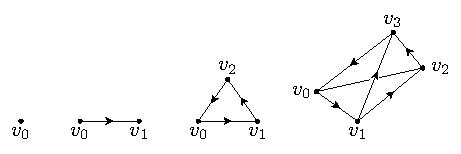
\includegraphics[scale=1.5]{images/fig_1.pdf}\\
                Figura \thefigcount. $n$ simplejos para $n=0,1,2$ y $3$.
                \stepcounter{figcount}
            \end{center}
        \end{minipage}

        De izquierda a derecha se muestran como serían el 0-simplejo, 1-simplejo, 2-simplejo y 3-simplejo metidos en $\mathbb{R}^3$.
    \end{obs}

    \begin{exa}
        El $n$-simplejo que contiene a los vectores canónicos $e_1,...,e_n$ y al cero en $\mathbb{R}^m$ es el conjunto:
        \begin{equation*}
            \Delta^n=\left\{(t_0,...,t_n)\in\mathbb{R}^{ n+1}\Big|\sum_{ i=0}^n t_i\textup{ y }t_i\geq0\textup{ }\forall i=0,...,n \right\}
        \end{equation*}
        es llamado \textbf{$n$-simplejo estándar}. Notemos que $\Delta^n=[0,e_1,...,e_n]$ donde $O$ es el origen de $\mathbb{R}^{ n+1}$.
    \end{exa}

    En homología va a resultar importante mantener el orden de los vértices del simplejo, por lo que cuando digamos \textit{$n$-simplejo}, realmente estaremos diciendo \textit{$n$-simplejo con un ordenamiento de vértices}.

    Una consecuencia de ordenar los vértices de un simplejo $[v_0,...,v_n]$ es que éstos determinan la orientación de los vértices $[v_i,v_j]$ de acuerdo a los subíndices ordenados de forma creciente.

    Especificar este orden de los vértices determina un homomorfismo lineal del $n$-simplejo estándar en cualquier otro $n$-simplejo $[v_0,...,v_n]$ que preserve el orden de los vértices, a saber:
    \begin{equation*}
        (t_0,...,t_n)\mapsto \sum_{ i=0}^n t_iv_i
    \end{equation*}
    los coeficientes $t_i$ son llamados $i$-ésimas \textbf{coordenadas baricéntricas} del punto $\sum_{ i=0}^n t_iv_i$ en el simplejo $[v_0,...,v_n]$.

    \begin{mydef}
        Sea $[v_0,...,v_n]$ un $n$-simplejo y tomemos $j=0,...,n$. Entonces el simplejo $[v_0,...,\hat{v_j},...,v_n]$ es un $(n-1)$-simplejo llamado \textbf{$j$-ésima cara de $[v_0,...,v_n]$}.
    \end{mydef}

    \begin{obs}
        Bajo la definición que hicimos anteriormente, todo subsimplejo de un simplejo estará siempre con los vértices ordenados de forma creciente, de acuerdo al orden que establecimos en el simplejo original. 
    \end{obs}

    \begin{mydef}
        El conjunto formado por la unión de todas las caras de un simplejo $\Delta^n$ es la \textbf{frontera de $\Delta^n$} y se denota por $\partial\Delta^n$. El \textbf{simplejo abierto} $\mathring{\Delta}^n$ es el conjunto $\Delta^n\setminus\partial\Delta^n$.
    \end{mydef}

    \begin{mydef}
        Una \textbf{estructura de $\Delta$-complejo en un espacio $X$} (o llamado simplemente \textbf{$\Delta$-complejo}) es una colección $\left\{\cf{\sigma_\alpha}{\Delta^{ n_\alpha}}{X} \right\}_{\alpha\in I}$ (con $n_\alpha\in\mathbb{N}\cup\left\{0 \right\}$ para todo $\alpha\in I$) tal que:
        \begin{enumerate}[label = \textit{(\arabic*)}]
            \item Para todo $\alpha\in I$, la reestricción $\sigma_\alpha\big|_{\mathring{\Delta}^{ n_\alpha}}$ es inyectiva, y todo punto de $X$ es la imagen de exactamente una reestriccion $\sigma_\alpha\big|_{\mathring{\Delta}^{ n_\alpha}}$.
            \item Para todo $\alpha\in I$ y para cada reestricción de $\sigma_\alpha$ a alguna cara de $\Delta^{ n_\alpha}$ existe $\beta\in I$ tal que esta reestricción coincide con $\cf{\sigma_\beta}{\Delta^{ n_\alpha-1}}{X}$ (donde $n_\beta=n_\alpha-1$).
            \item $A\subseteq X$ es abierto si y sólo si $\sigma_\alpha^{-1}(A)$ es abierto en $\Delta^{n_\alpha}$ para todo $\alpha\in I$.
        \end{enumerate}
    \end{mydef}

    \begin{obs}
        En el inciso \textit{(2)} identificamos cada cara de $\Delta^n$ con $\Delta^{ n-1}$ mediante el homomorfismo lineal entre ellos que preserva la orientación.
    \end{obs}

    La condición \textit{(3)} nos quita la condición trivial de que todos los puntos de $X$ sean vértices de algún simplejo.

    Una consecuencia inmediata de todas estas condiciones es que un espacio $X$ puede ser construido a partir de una colección de simplejos disjuntos $\Delta_\alpha^{n_\alpha}$, uno por cada $\cf{\sigma_\alpha}{\Delta^{ n_\alpha}}{X}$, el espacio obtenido a partir de identificar cada cara de $\Delta_\alpha^{ n_\alpha}$ con el correspondiente $\Delta_\beta^{ n_\alpha-1}$, correspondeinte a la reestricción de $\sigma_\beta$ de $\sigma_\alpha$ de la cara en cuestión.

    Para nuestro caso, basta con analizar por ejemplo al Toro:

    \begin{exa}
        %TODO Poner analisis del toro y definir sobre él una estructura de $\Delta$ complejo.
    \end{exa}

    \subsection{Homología Simplicial}

    Nuestro objetivo ahora es definir los grupos de homología de un $\Delta$-complejo $X$. Para ello, será imprescindible contar con todo lo hecho en la teoría sobre grupos libres y grupos abelianos libres.

    \begin{mydef}
        Sea 
    \end{mydef}

    \section{Homología Singular}

    Con lo hecho en la parte de homología simplicial, resultará un poco más sencillo observar qué es lo que está sucediendo en homología singular. En esta sección se dan definiciones y algunas otras propiedades básicas.

    \subsection{Definición de los grupos cúbicos singulares de homología}

    \begin{obs}
        De ahora en adelante $I=[0,1]$ denotará a este intervalo. Además, convenimos en que $I^0$ es un conjunto con un sólo punto, a saber $I^0=\left\{0\right\}$. Además, el conjunto $\mathbb{N}^*$ denotará a $\mathbb{N}\cup\left\{0\right\}.$
    \end{obs}

    \begin{mydef}
        Sea $X$ un espacio topológico. Si existe $n\in\mathbb{N}$ tal que $X\cong I^n$, diremos que $X$ es un \textbf{cubo $n$-dimensional}.
    \end{mydef}

    \begin{mydef}
        Sea $X$ espacio topológico y $n\in\mathbb{N}^*$ \textbf{$n$-cubo singular en $X$} es una función continua $\cf{T}{I^n}{X}$. 
    \end{mydef}

    \begin{exa}
        Si $n=0$, entonces $\cf{T}{\left\{* \right\}}{X}$ es una función que manda un punto en un punto.

        Si $n=0$, entonces $\cf{T}{I}{X}$ es un camino con puntos extremos $T(0)$ y $T(1)$.
    \end{exa}

    \begin{obs}
        Note que a diferencia de la parte de homología simplicial, en esta parte permitimos que nuestro mapeo $T$ no necesariamente sea lineal, ya que en la parte anterior se deduce rápidamente que $\Delta^n\cong I^n$.

        Más aún, esta es llamada homología singular ya que puede que la función $T$ tenga singularidades.
    \end{obs}

    Esta generalización nos permitirá hacer la construcción de la homología singular de forma similiar a como se hizo anteriormente.

    \begin{mydef}
        Sean $X$ espacio topológico y $n\in\mathbb{N}^*$. El conjunto $Q_n(X)$ denota al grupo abeliano libre generado por el conjunto de todos los $n$-cubos singulares en $X$.
    \end{mydef}

    \begin{obs}
        Un elemento de $Q_n(X)$ (dados como en la definición anterior) es de la forma:
        \begin{equation*}
            n_1T_1+n_2T_2+\cdots+n_kT_k
        \end{equation*}
        donde $n_i\in\mathbb{Z}$, $\cf{T_i}{I^n}{X}$ es función continua, para todo $i\in\natint{1,n}$ y $T_j\neq T_i$, para todo $i,j\in\natint{1,n}$ con $i\neq j$. La suma NO es la suma usual de funciones (pues puede que $X$ no tenga estructura que le permita realizar esta suma de funciones, y aunque tuviese, ignoraríamos este hecho), es únicamente usada para expresar a los elementos del grupo abeliano libre.
    \end{obs}

    \begin{mydef}
        Sean $X$ espacio topológico y $n\in\mathbb{N}$. Un $n$-cubo singular $\cf{T}{I^n}{X}$ es \textbf{degenerado} si existe $i\in\natint{1,n}$ tal que:
        \begin{equation*}
            T(x_1,...,x_{ i_1},...,x_n)=T(x_1,...,x_{ i_2},...,x_n)
        \end{equation*}
        para todo $x_{i_1},x_{i_2}\in I$. En otras palabras, $T$ no depende de la $i$-ésima entrada.
    \end{mydef}

    Notemos que admitimos que ningún $0$-cubo singular puede ser degenerado. Además, un $1$-cubo singular es dengerado si y sólo si es la función constante.

    \begin{mydef}
        Sean $X$ espacio topológico y $n\in\mathbb{N}$. $D_n(X)$ denota al subgrupo de $Q_n$ generado por el conjunto de todos los $n$-cubos singulares degenerados. Este es un subgrupo normal de $Q_n(X)$ (ya que es un subgrupo de un grupo abeliano), denotamos por:
        \begin{equation*}
            C_n(X)=Q_n(X)/D_n(X)
        \end{equation*}
        este es llamado \textbf{grupo de todas las cadenas singulares de $n$-cubos} o simplemente \textbf{$n$-cadenas de $X$}.
    \end{mydef}

    En otras palabras, lo que estamos haciendo es quitar al grupo de todos los $n$-cubos singulares a aquellos que deberían tener \textit{menos volumen} que los demás dentro de esta lista.

    Convenimos en que si $X=\emptyset$, entonces $Q_n(X)=D_n(X)=C_n(X)=\langle0\rangle$ para todo $n\in\mathbb{N}^*$.

    \begin{exa}
        Si $X=\left\{*\right\}$, entonces sólo puede haber un único cubo singular en $X$ para todo $n\in\mathbb{N}^*$. Además, este siempre es degenerado si $n\in\mathbb{N}$.

        Por tanto, $C_0(X)$ es cíclico infinito ya que $Q_0(X)$ lo es y $D_0(X)=\gen{0}$. Si $n\in\mathbb{N}$ se tiene que $C_n(X)=\gen{0}$ ya que $Q_n(X)=D_n(X)$.
    \end{exa}

    \begin{exa}
        Podemos ir más allá en la primer parte del ejemplo anterior, ya que para cualquier espacio $X$ se tiene que $D_0(X)=\gen{0}$, por lo que $C_0(X)=Q_0(X)$.
    \end{exa}

    \begin{exa}
        Para cualquier espacio $X$, $C_n(X)$ (con $n\in\mathbb{N}$) es grupo abeliano libre generado en el conjunto de todos los $n$-cubos singulares no dengenerados en $X$.
    \end{exa}

    \subsection{Caras de un cubo singular}

    Nuestro objetivo ahora es el de definir las caras de estos $n$-cubos singulares, de forma análoga a como se hizo con los simplejos.

    \begin{mydef}
        Sean $X$ espacio topológico y $n\in\mathbb{N}$. Sea $T$ un $n$-cubo singular en $X$, para cada $i\in\natint{1,n}$ se definen los $n$-cubos singulares:
        \begin{equation*}
            \cf{A_i(T),B_i(T)}{I^{ n-1}}{X}
        \end{equation*}
        dados por:
        \begin{equation*}
            \begin{split}
                A_iT(x_1,...,x_n)&=T(x_1,...,x_{ i-1},1,x_i,...,x_n)\\
                B_iT(x_1,...,x_n)&=T(x_1,...,x_{ i-1},0,x_i,...,x_n)\\
            \end{split}
        \end{equation*}
        $A_iT$ es llamada la \textbf{$i$-ésima cara frontal de $T$} y $B_iT$ es la \textbf{$i$-ésima cara trasera de $T$}.
    \end{mydef}

    \begin{obs}
        Podemos ver a $\cf{A_i}{Q_n(X)}{Q_{ n-1}(X)}$ y $\cf{B_i}{Q_n(X)}{Q_{ n-1}(X)}$ como funciones para cada $i\in\natint{1,n}$.
    \end{obs}

    Rápidamente (ejercicio), es posible verificar para cada $i,j\in\natint{1,n}$, $i< j$ y $n>1$:
    \begin{equation}
        \label{faceConmutativeIdentities}
        \begin{split}
            A_iA_j(T)&=A_{ j-1}A_i(T)\\
            B_iB_j(T)&=B_{ j-1}B_i(T)\\
            A_iB_j(T)&=B_{ j-1}A_i(T)\\
            B_iA_j(T)&=A_{ j-1}B_i(T)\\
        \end{split}
    \end{equation}

    \newcommand{\bound}[1]{\textup{\partial\left(#1\right)}}

    \begin{mydef}
        Sean $X$ espacio topológico y $n\in\mathbb{N}$. Para cada $n$-cubo singular $T$ se define:
        \begin{equation*}
            \partial_n(T)=\sum_{ i=1}^n (-1)^i\left[A_iT-B_iT \right]
        \end{equation*}
        Extendemos de forma natural $\partial_n$ al $Q_n$, definiéndolo en función de su valor en los elementos generadores. Denotamos esta extensión de igual manera y es tal que $\cf{\partial_n}{Q_n}{Q_{n-1}}$. Este es un homomorfismo llamado \textbf{operador frontera}.

        Por comodidad, denotaremos a este operador simplemente por $\partial$.
    \end{mydef}

    \begin{propo}
        Sea $n\in\mathbb{N}$ con $n>1$ y $T$ un $n$-cubo singular. Entonces:
        \begin{equation*}
            \partial_{ n-1}\left(\partial_n\left(T\right) \right)=0
        \end{equation*}
        Además, si $T$ es degenerado, entonces $\partial_n\left(T\right)\in D_{ n-1}(X)$. En otras palabras, $\partial_n(D_n(X))\subseteq D_{n-1}$. 
    \end{propo}

    \begin{proof}
        Probaremos primero la primera identidad. Veamos que:
        \begin{equation*}
            \begin{split}
                \partial_{ n-1}\left(\partial_n\left(T\right) \right)&=\partial_{ n-1}\left(\sum_{ i=1}^n (-1)^i\left[A_iT-B_iT \right] \right)\\
                &=\sum_{ i=1}^n (-1)^i\left[\partial_{ n-1}\left(A_iT\right)-\partial_{ n-1}\left(B_iT\right)\right]\\
                &=\sum_{ i=1}^n (-1)^i\left[\sum_{ j=1}^{n-1} (-1)^j\left[A_jA_iT-B_jA_iT \right]-\sum_{ j=1}^{n-1} (-1)^j\left[A_jB_iT-B_jB_iT \right]\right]\\
                &=\sum_{ i=1}^n \sum_{ j=1}^{n-1}(-1)^{i+j} \left[A_jA_iT-B_jA_iT-A_jB_iT+B_jB_iT\right]\\
            \end{split}
        \end{equation*}
        Analizaremos las sumas una por una:
        \begin{equation*}
            \begin{split}
                \sum_{ i=1}^n \sum_{ j=1}^{n-1}(-1)^{i+j}A_jA_iT&=\sum_{ i=1}^{ n-1}\sum_{ j=1}^{n-1}(-1)^{i+j}A_jA_iT+\sum_{ j=1}^{n-1}(-1)^{n+j}A_jA_nT\\
                &=\sum_{ j=1}^{n-1}(-1)^{1+j}A_jA_1T+\sum_{ j=1}^{n-1}(-1)^{2+j}A_jA_2T+\cdots+\\
                &+\sum_{ j=1}^{n-1}(-1)^{n-1+j}A_jA_{ n-1}T+\sum_{ j=1}^{n-1}(-1)^{n+j}A_jA_nT\\
            \end{split}
        \end{equation*}
        Hay dos casos, $n$ es par o $n$ es impar. Analicemos por casos:
        \begin{itemize}
            \item Suponga que $n$ es impar, entonces existe $k\in\mathbb{N}$ tal que $n=2k+1$, luego hay $2k$ sumandos. Hacemos:
            \begin{equation*}
                \begin{split}
                    \sum_{ i=1}^n \sum_{ j=1}^{n-1}(-1)^{i+j}A_jA_iT&=\sum_{ j=1}^{n-1}(-1)^{1+j}A_jA_1T+\sum_{ j=1}^{n-1}(-1)^{2+j}A_jA_2T+\cdots+\sum_{ j=1}^{n-1}(-1)^{k+j}A_jA_{k}T+ \\
                    &+\sum_{ j=1}^{n-1}(-1)^{k+1+j}A_jA_{k+1}T+\sum_{ j=1}^{n-1}(-1)^{n-1+j}A_jA_{ n-1}T+\cdots+\sum_{ j=1}^{n-1}(-1)^{n+j}A_jA_nT\\
                \end{split}
            \end{equation*}
            Veamos que todo elemento de una suma de las primeras $k$-sumas se cancela con alguno de las otras $k$-sumas que siguen. En efecto, considere el sumando $(-1)^{l+j}A_jA_lT$ con $l\in\natint{1,n}$.
        \end{itemize}
    \end{proof}



    \newpage

    \section{Ejercicios}

    \subsection{Homología Simplicial}

    \subsection{Homología Singular}

    \begin{excer}
        Compute $\partial_n(T)$ para el caso en que $n=1,2$.
    \end{excer}


\end{document}